\subsection{Ablation study for GCF}
Meng Liu et. al does not present an ablation study for BiTGCF and GCF, which LightGCN showed is important with their regards to NGCF \cite{lightgcn,BiTGCF}.
In this section we conduct an ablation study on GCF to get an understanding on the effect of the different parts of the embedding propagation and layer combination.
\autoref{fig:GCF-NDCG-ablation-study} and \autoref{fig:GCF-recall-ablation-study} contains the GCF ablation study, where all GCF modifications still have the inner product between users and items, except for LightGCN.
The methods are as described here:\\
\textcolor{red}{(We might also be required to test this with dropout to prevent overfitting on the methods that utilizes concatenation as layer combination, and see what effect this has on the results.)}
\begin{itemize}
    \item \textbf{GCF}: The original GCF method as described in \autoref{subsubsec:GCF-embed-propagation}.
    \item \textbf{GCF-minus-self-con}: GCF where self connection has been removed.
    \item \textbf{GCF-sum}: GCF where the layer combination has been changed to weighted summation instead of concatenation.
    \item \textbf{GCF-sum-minus-self-con}: GCF with removed self connection and weighted summation as layer combination.
    \item \textbf{GCF-minus-IP}: GCF where inner product has been removed. \textcolor{red}{results missing}
    \item \textbf{GCF-minus-IP-and-self-con}: GCF without inner product and self connections. \textcolor{red}{results missing}
    \item \textbf{LightGCN}: Original LightGCN as described in \autoref{subsubsec:LightGCN-embed-propagation}.
    \item \textbf{LightGCN-self-con}: LightGCN with self connections.\textcolor{red}{results missing}
    \item \textbf{LightGCN-concat}: LightGCN with concatenation as layer combination. \textcolor{red}{results missing}
\end{itemize}

\begin{figure}[h!]
    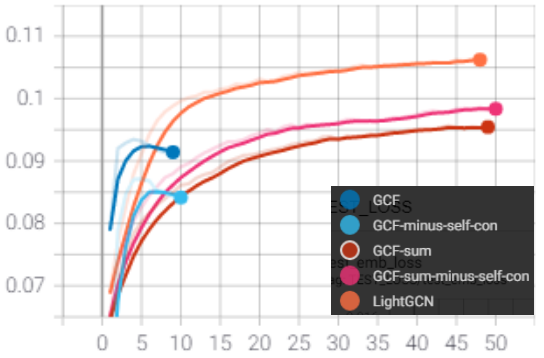
\includegraphics[width=\linewidth]{figures/GCF-NDCG-Yelp-ablation.png}
    \caption{NDCG@50 for the Yelp2020 dataset.}
    \label{fig:GCF-NDCG-ablation-study}
\end{figure}

\begin{figure}[h!]
    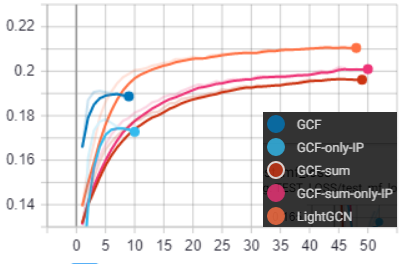
\includegraphics[width=\linewidth]{figures/GCF-recall-Yelp-ablation.png}
    \caption{Recall@50 on the Yelp2020 dataset.}
    \label{fig:GCF-recall-ablation-study}
\end{figure}
From \autoref{fig:GCF-NDCG-ablation-study} and \autoref{fig:GCF-recall-ablation-study} it can be seen that the methods that does not utilize concatenation as layer combination performs worse than the methods that utilize summation.
For these experiments the dropout ratio is 0, so it could be because the concatenation methods hits overfitting.
Additionally we can see that self connections are beneficial, when using concatenation as layer combination, but decreases performance when using weighted summation as layer combination.
This is probably because that with weighted summation, the self connection are implicit added with the initial $e_u^{(0)}$ and $e_i^{(0)}$ embeddings, as these represents the adjacency matrices.